\section{Experimentelles Setup}
Das folgende Kapitel verdeutlicht den Aufbau der Experimentierumgebung, die für die technische Durchführung benötigt wurde. Dabei wird auf Datensätze, Modelle und deren Strukturen, wie auch auf die Implementierung von Angriffsmethoden und Verteidigungsmaßnahmen eingegangen. Die Auswahl und Konfiguration dieser Elemente sind entscheidend für die Reproduzierbarkeit der Experimente sowie für die Validität und Aussagekraft der ausgearbeiteten Ergebnisse.
\subsection{Datensätze}\label{subsection:datensaetze}
%mnist
%celeba
%ffhq
In diesem Abschnitt werden die Datensätze vorgestellt, die als Grundlage für die Trainings- und Angriffsdurchführungen in dieser Forschungsarbeit dienen. Eine sorgfältige Auswahl und detaillierte Beschreibung dieser Datensätze sind von zentraler Bedeutung, um die Integrität der Experimente zu gewährleisten und eine solide Grundlage für die Analyse der Ergebnisse und Beobachtungen zu schaffen.

In dieser Arbeit wurde aus Gründen der Einfachheit der MNIST-Datensatz (\cite{noauthor_mnist_nodate}) verwendet, welcher eine präzise Abfolge von Ziffern repräsentiert. Dieser Datensatz umfasst verschiedene Datenpunkte, die den Klassen der Zahlen 0 bis 9 zugeordnet sind. 

\begin{figure}[H]
	\centering
	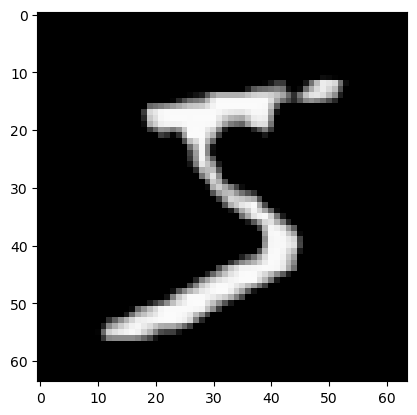
\includegraphics[width=0.3\linewidth]{Bilder/5_mnist.png}
	\caption{Beispielbild des MNIST-Datensatzes}
	\label{img:mnist}
\end{figure}

Die Datenpunkte sind in Form von sogenannten Ein-Kanal-Bildern repräsentiert, die vom menschlichen Auge in bestimmten Darstellungen als schwarz-weiß wahrgenommen werden (siehe Abbildung \ref{img:mnist}). Die Größe der Bilder, die zur Erstellung des Trainingsdatensatzes verwendet wurde, beträgt $64 \times 64$ Pixel. Dabei besitzt jeder Pixel einen normalisierten Wert zwischen 0 und 1, der die \glqq Farbe\grqq{} festlegt. Mit der Zusammensetzung aller Pixel entsteht das finale Bild.

Die Entscheidung für den MNIST-Datensatz wurde aufgrund seiner weiten Verbreitung in der Forschung und seiner klaren Struktur zur Repräsentation von Ziffern getroffen, wobei die Bildmerkmale vergleichsweise als \glqq einfach\grqq{} gelten. Die Fokussierung auf Zahlen im Bereich von 0 bis 9 ermöglicht eine gezielte Untersuchung spezifischer Klassen und vereinfacht die Interpretation der Ergebnisse. Dies erleichtert eine anschaulichere Analyse der durchgeführten Angriffe und liefert dem Betrachter klare und eindeutige Ergebnisse.

Der MNIST-Datensatz eignet sich besonders gut für die Evaluierung von Angriffen aufgrund seiner klaren Struktur und begrenzten Klassenanzahl. Dies ermöglicht eine präzise Bewertung der Wirksamkeit von Verteidigungsmaßnahmen und bietet gleichzeitig eine klare Vergleichsbasis für verschiedene Angriffsszenarien. Darüber hinaus hat sich gezeigt, dass auch komplexe Modelle wie das VGG16-Netzwerk auf Basis des MNIST-Datensatzes effizient trainiert werden können und bereits nach wenigen Epochen eine bemerkenswert hohe Genauigkeit auf Testdaten aufweisen.

Im Kontext neuronaler Netzwerke, die für die Generierung von Bildern eingesetzt werden, offenbart sich, dass diese rasch auf Grundlage des MNIST-Datensatzes angepasst werden können. Die Modelle generieren zügig Bilder, welche eine deutliche Ähnlichkeit zum Trainingsdatensatz aufweisen. Diese \glqq Einfachheit\grqq{} erweist sich als vorteilhaft für die transparente und effektive Analyse unterschiedlicher Angriffsstrategien sowie deren Auswirkungen auf die Bildgenerierung neuronaler Netzwerke.

Um eine weitere Validierungsebene für Versuchsdurchführungen bieten zu können, wurde der QMNIST-Datensatz (\cite{yadav_cold_2019}), der eine Rekonstruktion des MNIST-Datensatz ist, verwendet. Die Datenpunkte sind dabei nicht komplett identisch zu den jenigen des MNIST-Datensatzes und bieten somit die Möglichkeit, die Angriffe auf weitesgehend ungesehene Daten zu validieren.

Neben dem MNIST- wurde auch der CelebA-Datensatz (\cite{noauthor_celeba_nodate}) verwendet, der verschiedene Gesichtsbilder von 10.177 berühmten Personen in verschiedenen Klassen beinhaltet. Insgesamt hat er damit über 200.000 Bilder. Dieser eignet sich für verschiedene Use-Cases, wobei er in diesem Fall lediglich als Trainingsdatensatz für einen \glqq Personen\grqq-Klassifikator genutzt wurde. Auch hier werden die Bilder während des Ladens auf eine Größe von $64 \times 64$ Pixeln verändert und entstehen, im Gegensatz zu den MNIST-Bildern, aus 3 Kanälen. Auch hier wird jeder dieser Pixel auf einen normalisierten Wert zwischen 0 und 1 transformiert. Dabei wird jeweils rot, grün und blau von einem bestimmten Kanal repräsentiert. 

Der CelebA-Datensatz wurde als Vergleichsdatensatz zum zuvor genannten MNIST-Datensatz ausgewählt. Dies geschah sowohl, um Angriffe auf komplexere Datensätze zu prüfen, als auch, um Black-Box-Angriffe basierend auf einen bezüglich des CelebA-Datensatz trainierten Klassifizierer auf Grundlage eines anderen Gesichtsdatensatzes (\cite{noauthor_nvlabsffhq-dataset_2023}) zu erforschen. Diese Entscheidung ermöglichte die Simulation verschiedener Angriffsszenarien, die diverse Strategien und Durchführungsprozesse umfassen.

\begin{figure}[H]
	\centering
	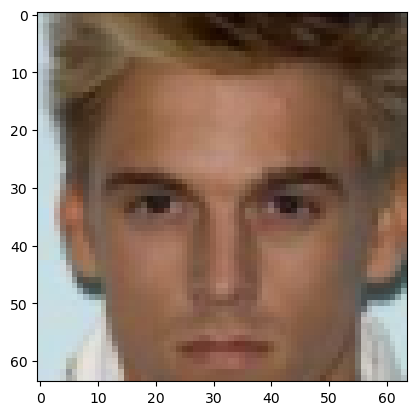
\includegraphics[width=0.3\linewidth]{Bilder/0_celeba_one.png}
	\caption{Beispielbild des CelebA-Datensatzes}
	\label{img:celeba}
\end{figure}

Die vielseitige Nutzung des CelebA-Datensatzes erstreckte sich über verschiedene Trainingsparadigmen. Einerseits wurde der Datensatz zur Schulung von Klassifikatoren herangezogen, die auf der VGG16-Architektur basierten. Andererseits wurde er auch für das Training eines herkömmlichen DCGAN-Netzwerks verwendet, um die Generierung von \glqq neuen\grqq{} Gesichtsbildern zu ermöglichen. Dies ermöglichte die Evaluierung der Anfälligkeit von Modellen unterschiedlicher Architekturen gegenüber Angriffen und trug zur Erweiterung des Verständnisses für die Sicherheit von Gesichtsdatensätzen bei.

Neben den Hauptdatensätzen CelebA und MNIST wurde der FFHQ-Datensatz (\cite{noauthor_nvlabsffhq-dataset_2023}) in dieser Arbeit integriert. Die \glqq rohen\grqq{} Bilddaten dieses Datensatzes weisen eine beeindruckende Größe von $1024 \times 1024$ auf und repräsentieren qualitativ hochwertige Bilder. Der FFHQ-Datensatz wurde eingeführt, um die Untersuchungen auf realistische Gesichtsbilder und einen unbekannten Datensatz zu erweitern. Hierbei wurde ein vortrainiertes Style-GAN Netzwerk auf Basis dieses Datensatzes verwendet, um realistische Gesichtsbilder zu generieren.

\begin{figure}[H]
	\centering
	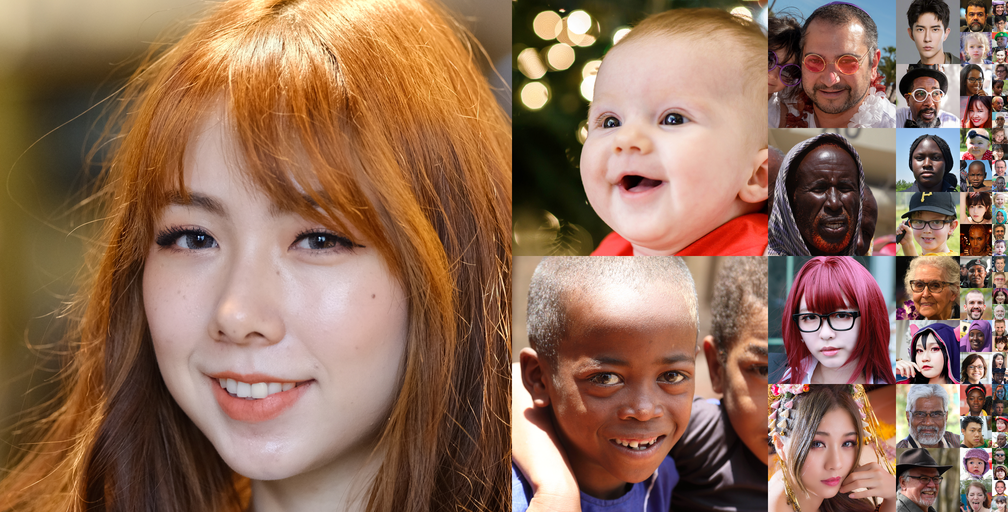
\includegraphics[width=0.7\linewidth]{Bilder/ffhq.png}
	\caption{Beispielbilder des Flickr-Faces-HQ-Datensatzes}
	\label{img:ffhq}
\end{figure}

Das Style-GAN Netzwerk, basierend auf dem FFHQ-Datensatz, ermöglichte nicht nur die Erstellung von hochqualitativen Gesichtsbildern, sondern trug auch zur Erweiterung der Vielfalt in den untersuchten Merkmalen bei. Im Gegensatz zu CelebA bietet der FFHQ-Datensatz eine breitere Auswahl an Herkunft, Altersgruppen und anderen charakteristischen Merkmalen.

Die Integration des FFHQ-Datensatzes eröffnete die Möglichkeit, reale Bildqualität in die Evaluierung von Angriffsszenarien einzubeziehen. Die repräsentativen Bilder des FFHQ-Datensatzes förderten die präzise Analyse von Angriffen auf hochauflösende und vom Zielmodell ungesehene Gesichtsbilder und trugen zur Entwicklung eines umfassenderen Verständnisses der Sicherheit von Gesichtsdatensätzen bei.

\subsection{Modelle}
%VGG16
%DCGAN
%StyleGAN
Die \textit{Architektur} der eingesetzten Modelle spielt eine zentrale Rolle in der Experimentierumgebung. Hier werden die gewählten Modelle hinsichtlich ihrer Struktur und Hyperparameter, die während des Traininsprozesses verwendet wurden, detailliert beschrieben. Eine genaue Vorstellung der Modelle ist entscheidend, um nachvollziehen zu können, wie diese auf die Datensätze angewendet wurden und welche Rolle sie in den folgenden Angriffs- und Verteidigungsszenarien spielen.

Die essentielle Architektur, die als Grundlage für den Klassifizierer dient, ist das VGG-16 Netzwerk (\cite{simonyan_very_2015}), ein CNN, das in der Bilderkennung eingesetzt wird. Dieses Netzwerk folgt dem Prinzip der \glqq Very Deep Convolutional Networks\grqq{} und zeichnet sich durch herausragende Merkmalsextraktionseigenschaften aus, wodurch es besonders für Bildklassifikationsaufgaben geeignet ist. Die Struktur setzt sich durch die sequenzielle Anordnung verschiedener Schichten zusammen, darunter Fully-Connected-, Pooling- und Convolutional-Schichten.
Das VGG-16 Netzwerk besteht insgesamt aus 16 Schichten, von denen 13 Convolutional- und 3 Fully-Connected-Schichten sind. Diese Schichten ermöglichen eine tiefgehende und hierarchische Repräsentation von Merkmalen, beginnend mit einfachen lokalen Strukturen bis hin zu abstrakteren und komplexeren Konzepten im Verlauf der Schichtfolge. Hervorzuheben ist, dass die Convolutional-Schichten Filter mit einer Größe von 3x3 Pixeln und einer Schrittweite von 1 Pixel verwenden, die Max-Pooling-Schichten eine Größe von 2x2 Pixeln und eine Schrittweite von 2 Pixeln aufweisen, und die Aktivierungsfunktion in allen Schichten, bis auf die finale Klassifikationsschicht, die ReLU-Funktion ist. 
\begin{equation}
	Relu(z) = max(0, z)
\end{equation}
Während des Vorwärtsdurchlaufs eines bestimmten Datenpunkts sind die Convolutional-Schichten maßgeblich für die Extraktion von Merkmalen verantwortlich.
Die Integration der vollvermaschten Schichten im Netzwerk fügt extrahierte Merkmale zusammen, um diese in der abschließenden Schicht des Bildklassifikators interpretieren zu können. Das Resultat ist ein Vektor, dessen Länge der Anzahl der Klassen im Datensatz entspricht, und der durch die Softmax-Aktivierungsfunktion erzeugt wird. 
\begin{equation}
	\sigma(z_i) = \frac{e^{z_{i}}}{\sum_{j=1}^K e^{z_{j}}} \ \ \ for\ i=1,2,\dots,K
\end{equation}
Diese Klassifikation erfolgt auf Basis eines personalisierten Headers, der eine vollvermaschte Schicht mit der benannten Aktivierungsfunktion als Abschluss enthält. Die Neuronenanzahl dieser Schicht gleicht der Anzahl der Klassen im Datensatz.
Besondere Bedeutung kommt der Integration von Max-Pooling-Schichten in bestimmten Abschnitten des Netzwerks zu. Diese Schichten reduzieren die Merkmalskartengröße und erhöhen die Invarianz gegenüber kleinen Translationen im Eingabebild. Diese Struktur trägt dazu bei, die Robustheit des Modells zu steigern und seine Fähigkeit zur Erfassung invarianten Wissens zu stärken.
Hervorzuheben ist, dass das VGG-16 Netzwerk auf dem ImageNet-Datensatz trainiert wurde, der 1000 verschiedene Klassen von Objekten enthält. Die hohe Genauigkeit bei der Klassifizierung von Bildern macht es zu einem oft verwendeten vortrainierten Modell in verschiedenen Computer-Vision-Anwendungen. 

\textit{Anwendung} fand das neuronale Netzwerk, das auf der VGG-16 Netzarchitektur aufbaut, in zwei Klassifikationsmodellen, welche auf der einen Seite handgeschriebene Ziffern und auf der anderen Seite Gesichter berühmter Persönlichkeiten klassifizieren sollen. Trainiert wurde auf Basis der in \ref{subsection:datensaetze} beschriebenen MNIST- und CelebA-Datensätze.


%% muss noch überarbeitet werden
\begin{table}[h]
	\centering
	\renewcommand{\arraystretch}{1.5}
	\resizebox{\textwidth}{!}{
		\begin{tabular}{c|ccccc|c}
			\textbf{Datensatz} & \textbf{Lernrate} & \textbf{Epochenanzahl} & \textbf{Batch-Größe} & \textbf{Momentum} & \textbf{Weight-Decay} & \textbf{Genauigkeit bezüglich Testdaten}\\
			\hline
			\textit{CelebA} & 1e-3 & 100 & 256 & 0.9 & 5e-4 & \textbf{65,23\%}\\
			\hline
			\textit{MNIST} & 1e-3 & 15 & 64 & 0.9 & 1e-3 & \textbf{99,63\%}\\
			\hline
		\end{tabular}
	}
	\caption{Hyperparameter des \glqq normalen\grqq{} Trainings bezüglich der angegebenen Datensätze}
	\label{tab:nn_train}
\end{table}

\begin{figure}[H]
	\centering
	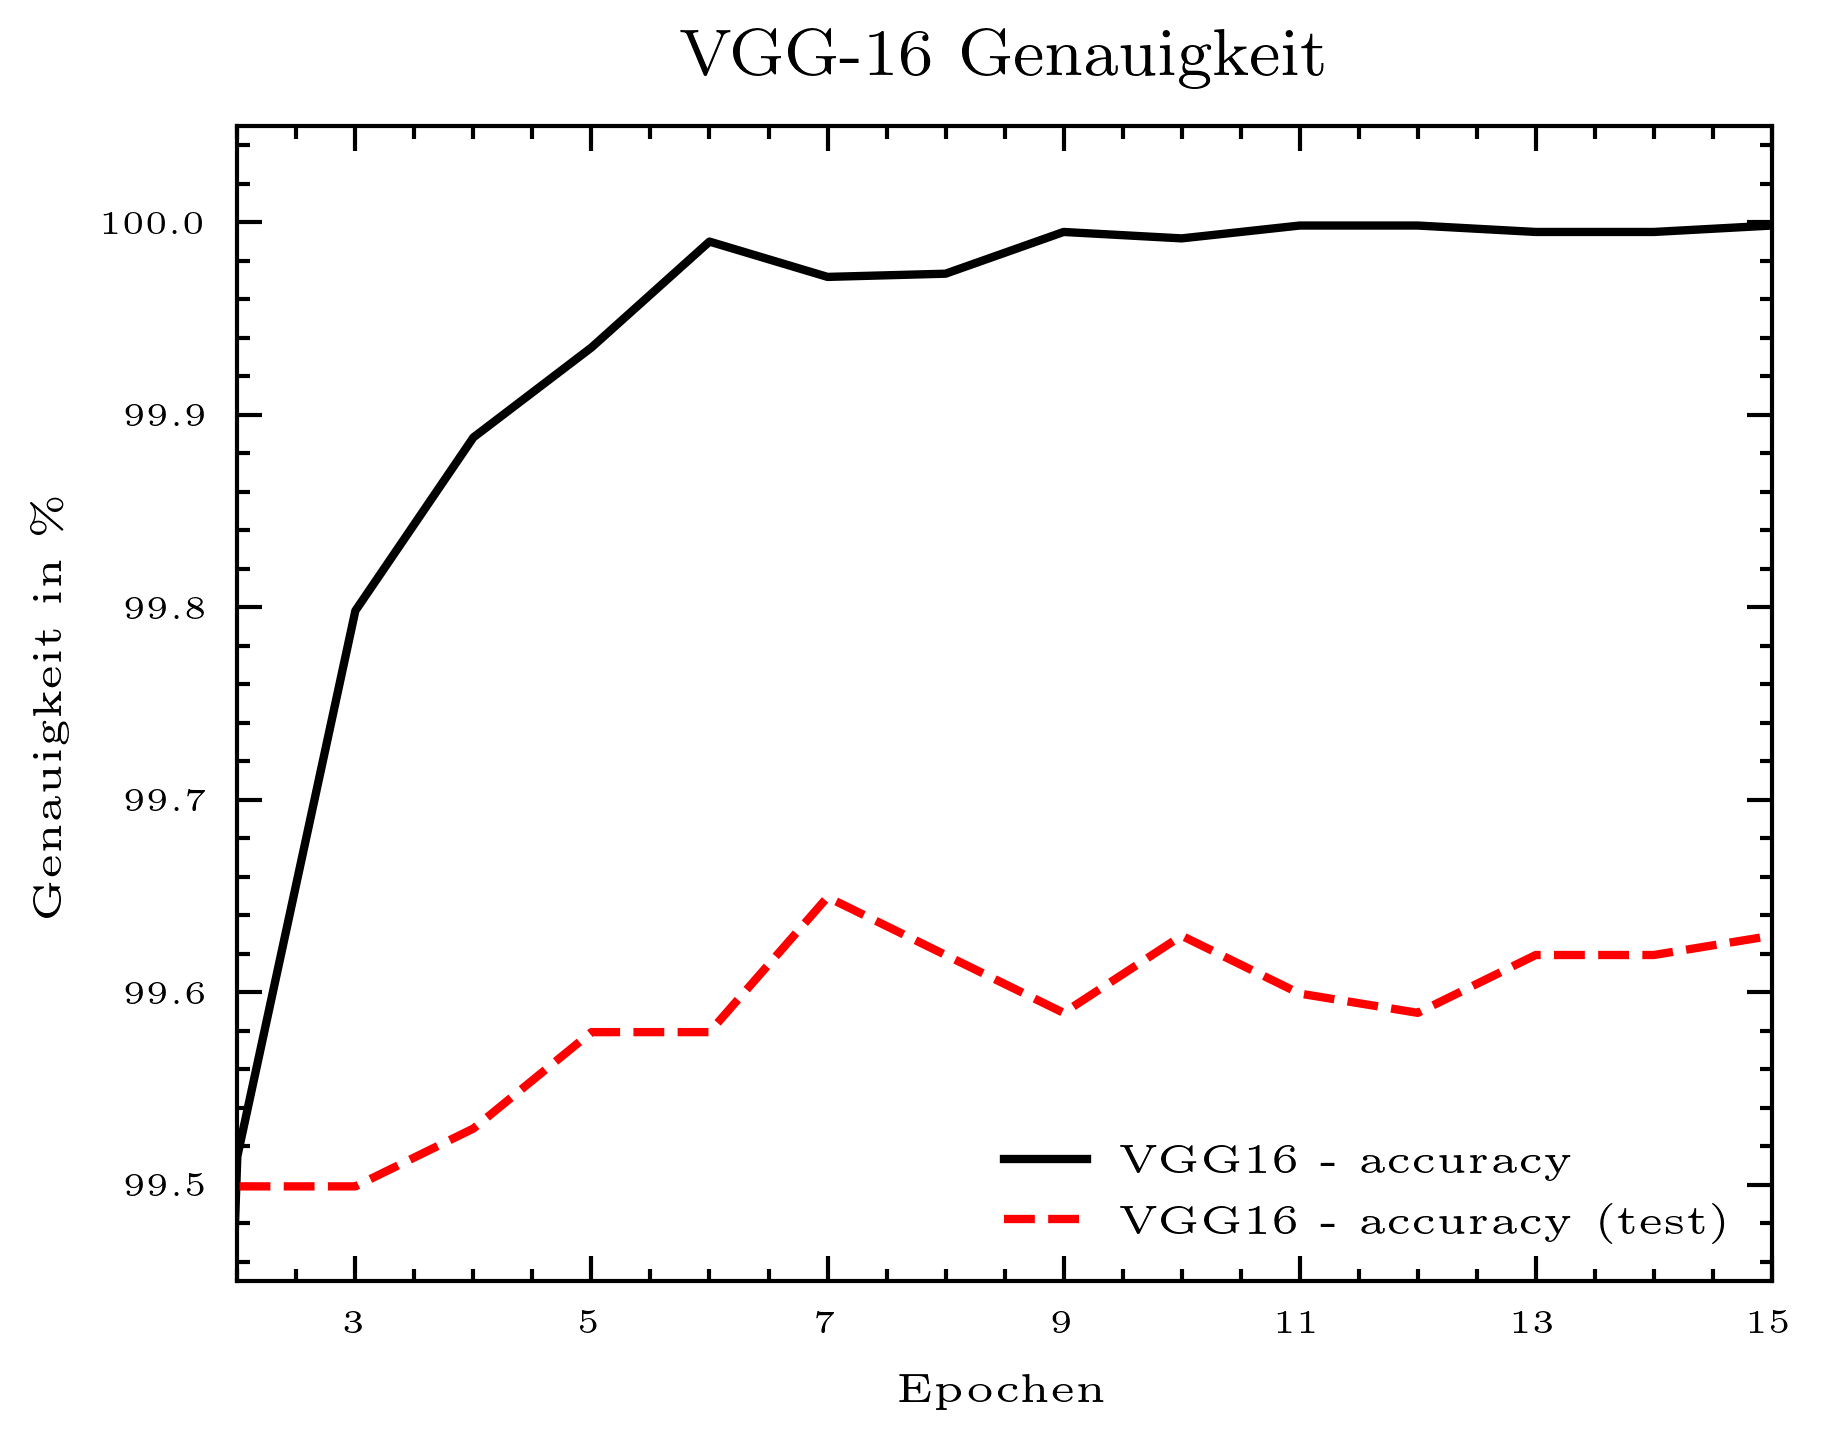
\includegraphics[width=0.5\linewidth]{Bilder/mnist_nn_acc.png}
	\caption{Genauigkeit während des Trainingsprozesses bezüglich Trainings- und Testdaten des MNIST-Datensatzes}
	\label{img:mnist_nn_acc}
\end{figure}

\begin{figure}[H]
	\centering
	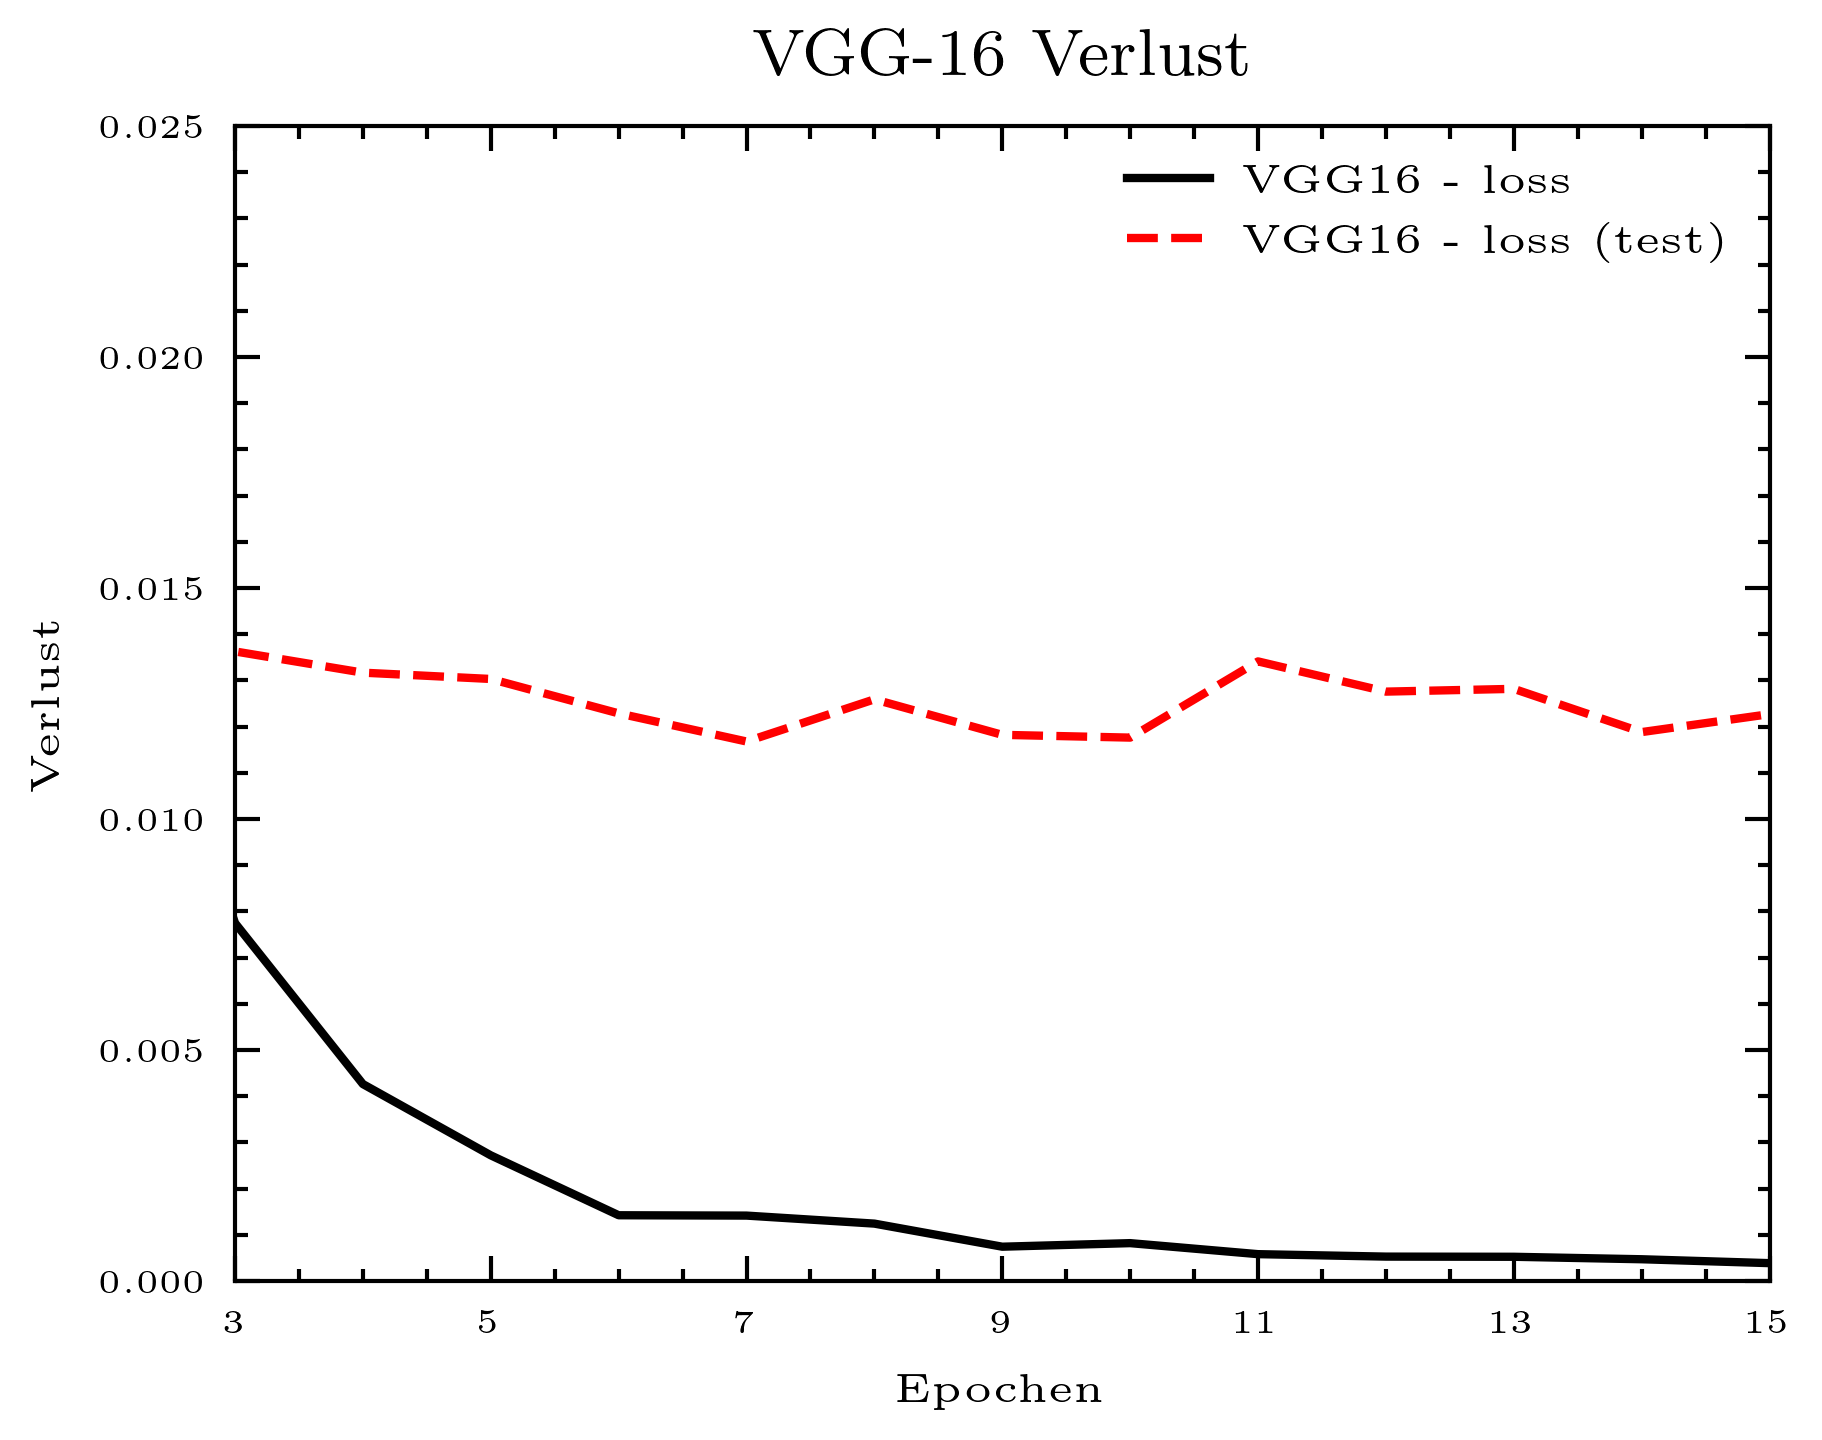
\includegraphics[width=0.5\linewidth]{Bilder/mnist_nn_loss.png}
	\caption{Verlust während des Trainingsprozesses bezüglich Trainings- und Testdaten des MNIST-Datensatzes}
	\label{img:mnist_nn_loss}
\end{figure}

% Trainingsteil des VGG hinzufügen 
Die Trainingsroutine des VGG-16 Netzwerks basiert auf einem überwachten Lernverfahren (siehe \ref{subsec:supervisedlearning}), wobei eine Menge an Datenpunkten des Trainingssatzes, welchen eine bestimmte Kategorisierung/ein bestimmtes Label zugeordnet ist, genutzt wird, um die Parameter des Modells möglichst effizient und zielführend zu aktualisieren. Dabei wurde bei der Durchführung dieser Arbeit kein Wert auf eine optimalisierte Modellgenauigkeit und Leistung gelegt, weshalb ein mögliches Hyperparameter-Tuning eine Verbesserung der Modellleistung herbeiführen kann. Die Durchführung des Trainings auf Basis verschiedener Datensätze (CelebA und MNIST) wurde mit verschiedenen Hyperparametereinstellungen ausgeführt, wie in Tabelle \ref{tab:nn_train} beschrieben.
\begin{figure}[H]
	\centering
	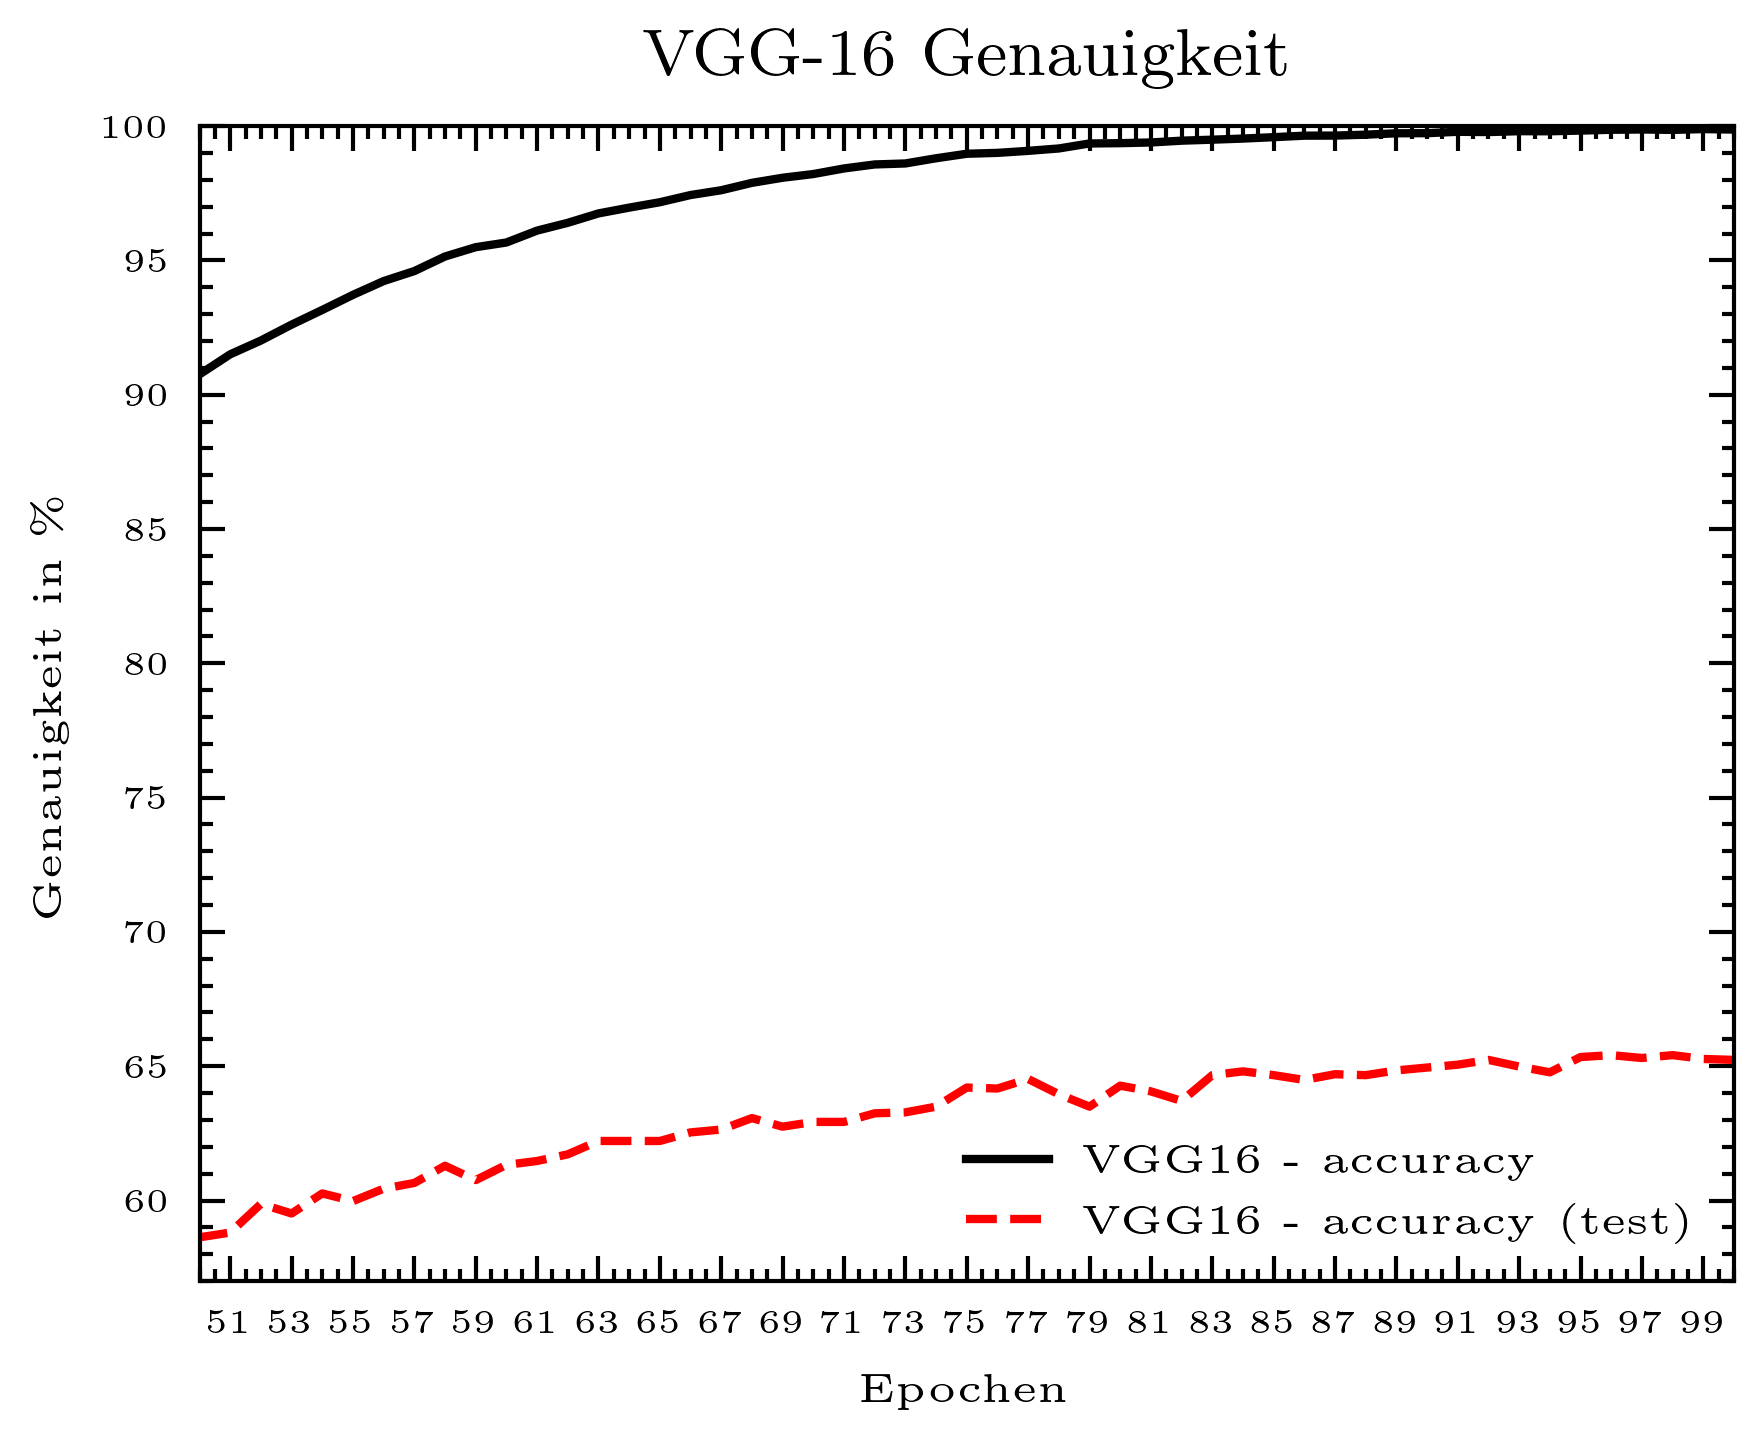
\includegraphics[width=0.5\linewidth]{Bilder/celeba_nn_acc.png}
	\caption{Genauigkeit während des Trainingsprozesses bezüglich Trainings- und Testdaten des CelebA-Datensatzes}
	\label{img:celeba_nn_acc}
\end{figure}

\begin{figure}[H]
	\centering
	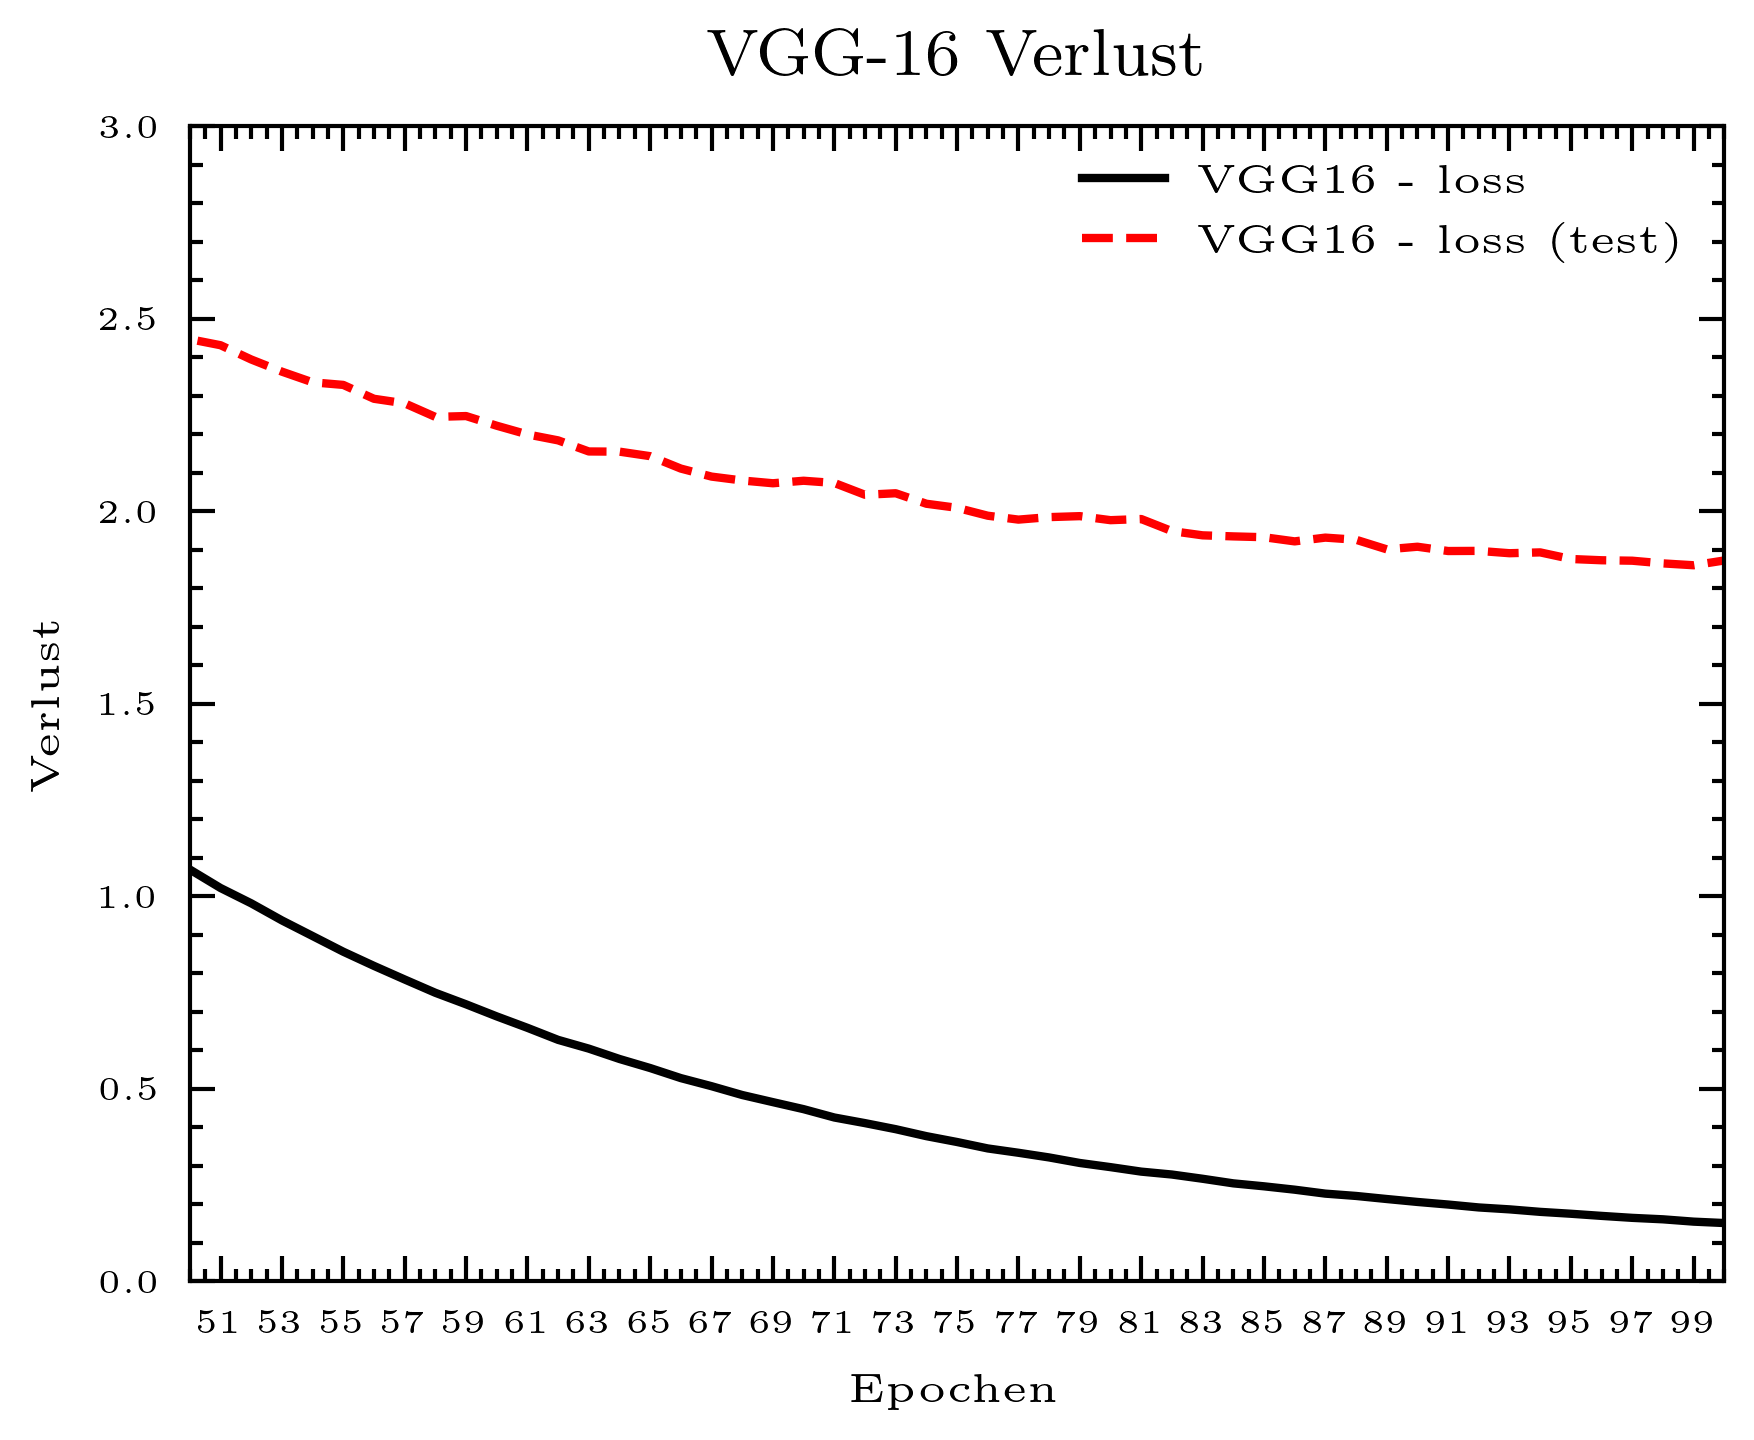
\includegraphics[width=0.5\linewidth]{Bilder/celeba_nn_loss.png}
	\caption{Verlust während des Trainingsprozesses bezüglich Trainings- und Testdaten des CelebA-Datensatzes}
	\label{img:celeba_nn_loss}
\end{figure}

 Deutlich zu erkennen ist, dass die Testgenauigkeit (Abbildung \ref{img:celeba_nn_acc}) des Modells bezüglich Gesichtdaten sehr niedrig ist, die Trainingsgenauigkeit allerdings deutlich höher. Auch der Verlust des Modells (Abbildung \ref{img:celeba_nn_loss}) während des Trainings ist sehr hoch und passt sich nur sehr langsam an. Dies ist auf den Aufbau des genutzten Datensatzes zurückzuführen, der aufgrund der großen Klassenanzahl (>1000) mit maximal 10 Bildern pro Klasse nicht für ein Training zur Klassifikation von Gesichtsbildern prominenter Persönlichkeiten geeignet ist. Durch die Divergenz zwischen Trainings- und Testgenauigkeit ist ersichtlich, dass es sich um ein sogenanntes Overfitting handelt, welches eine hohe Genauigkeit bezüglich der im Training verwendeten Daten aufweist, allerdings Testdaten nicht gut erkannt werden. Somit erkennt man ungefähr jedes 2. Bild richtig, was eine sehr schwache Modellleistung hervorhebt. Die Leistung des auf den MNIST-Datensatz trainierten VGG-16 Modells ist deutlich besser, da sowohl Test- als auch Trainingsgenauigkeit (Abbildung \ref{img:mnist_nn_acc}) an den Genauigkeitswert von 100\% konvergieren. Auch der Verlust des Modells konvergiert gegen 0 (Abbildung \ref{img:mnist_nn_loss}).

Zur Durchführung der im vorliegenden Kontext beschriebenen Modell-Inversions-Angriffe ist ein neuronales Netzwerk erforderlich, das die Fähigkeit besitzt, spezifische Bilder zu generieren. In diesem Zusammenhang wurde das Deep Convolutional Generative Adversarial Network (DCGAN) gemäß der Arbeit von Radford et al. (\cite{radford_unsupervised_2016}) eingesetzt. Dieses Netzwerk zeichnet sich durch eine Vielzahl von speziellen architektonischen Merkmalen aus. Es besteht primär aus zwei Hauptkomponenten: dem Generator, der die Generierung neuer Datenpunkte durch zufälliges Rauschen übernimmt, und dem Diskriminator, der versucht, zwischen realen und gefälschten Bildern zu differenzieren.

Ein zentraler Aspekt dieser Architektur ist die tiefe Faltungsstruktur, die sowohl im Generator als auch im Diskriminator Verwendung findet. Diese Struktur ermöglicht die Erfassung räumlicher Strukturen in den generierten Daten. Im Gegensatz zu herkömmlichen Convolutional Neural Networks (CNNs) werden in der Architektur von DCGANs keine Pooling-Schichten verwendet, um Unschärfe zu vermeiden. Stattdessen setzt man auf Normalisierungsschichten, um das Training stabil zu gestalten und die Konvergenz der Verlustfunktionen zu beschleunigen.

Eine weitere Abweichung von konventionellen CNNs besteht in der Verwendung der LeakyReLU-Aktivierungsfunktion anstelle der üblichen ReLU-Funktion.
\begin{equation}
	\text{LeakyReLU}(x) = \begin{cases}
		x, & \text{if } x > 0 \\
		\alpha x, & \text{otherwise}
	\end{cases}
\end{equation}
Hier repräsentiert $\alpha$ eine kleine, positive Konstante. Der Einsatz dieser modifizierten Aktivierungsfunktion zielt darauf ab, das Problem der \glqq tötenden Neuronen\grqq{} zu umgehen, das bei der Verwendung der ReLU-Aktivierungsfunktion auftreten kann. Dabei werden Neuronen während des Trainings inaktiv, weshalb kein positiver Beitrag zur Leistungssteigerung des Modells beigetragen wird. In bestimmten Fällen kann die Modellleistung dadurch sogar verschlechtert werden. 

Die Trainingseffizienz des DCGAN kann variieren, abhängig von der verwendeten Hardware. Es wird empfohlen, das Netzwerk auf einer oder mehreren GPUs zu trainieren, da diese leistungsfähiger sind als eine ausschließliche Verwendung der CPU. Eine alternative Möglichkeit besteht im Transfer Learning, bei dem ein bereits trainiertes Modell als Ausgangspunkt für das aktuelle Training dient. Allgemein lässt sich feststellen, dass mit zunehmenden Epochen eine Verbesserung der Qualität der neu generierten Bilder erkennbar ist.

%% muss noch überarbeitet werden
\begin{table}[h]
	\centering
	\renewcommand{\arraystretch}{1.5}
	\resizebox{\textwidth}{!}{
		\begin{tabular}{c|ccccc}
			\textbf{Datensatz} & \textbf{Lernrate} & \textbf{Epochenanzahl} & \textbf{Batch-Größe} & \textbf{Momentum} & \textbf{Bildgröße}\\
			\hline
			\textit{CelebA} & 2e-4 & 100 & 128 & 0.5 & 64 $\times$ 64\\
			\hline
			\textit{MNIST} & 2e-4 & 100 & 128 & 0.5 & 64 $\times$ 64 \\
			\hline
		\end{tabular}
	}
	\caption{Hyperparameter eines DCGAN-Trainings bezüglich der angegebenen Datensätze}
	\label{tab:dcgan}
\end{table}

% Trainingsteil des DCGAN hinzufügen 
Das DCGAN wurde auf Basis der in Tabelle \ref{tab:dcgan} aufgelisteten Hyperparametern trainiert. Dabei wurde darauf geachtet, dass generierte Bilder \glqq weitesgehend fehlerunbehaftet\grqq{} dargestellt werden. Dies bedeutet, dass Gesichter und Ziffern deutlich erkennbar und nicht mit großer Störung versehen sind. Jedoch wurde kein Augenmerk auf den Realitätsgrad des Bildes gelegt, sodass Generierungen von echten, hochaufgelösten Bildern deutlich zu unterscheiden sind. 
%%%% Hier muss das Training noch genauer beschrieben werden (mit Graph usw.)

Um die Angriffsszenarien erweitern zu können, wurde ein weiteres generatives Modell zur Erzeugung hochauflösender Gesichtsbilder verwendet. Dieses StyleGAN (\cite{karras_style-based_2019}) basiert auf dem Konzept der generativen adverariellen Netzwerke und umfass -- wie ein DCGAN -- sowohl Generator und Diskriminator. Hierbei generiert der Generator die neuen Bilder, die dann vom Diskriminator nach Qualität bewertet werden. Während des Trainings werden beide Komponenten verbessert, was qualitativ hochwertigere und realistischere Bilder mit sich bringt. Die StyleGAN-Architektur hat neben den realistischen Bildausgaben die Besonderheit, dass Stilvarationen in Generierungen gut zu kontrollieren sind. Dies bedeutet, dass bestimmte Merkmale, wie beispielsweise Mimik und Haarfarbe, separat manipuliert werden können, um dadurch individuelle Ergebnisse zu erzielen. Diese Art des GANs wurde nicht selbst trainiert, sondern vortrainiert von NVIDIA (\cite{noauthor_nvlabsstylegan_2024}) geladen.

Die Auswahl der genutzten Modelle, nämlich das VGG-16 Netzwerk, das Deep Convolutional Generative Adversarial Network (DCGAN) und das StyleGAN, erfolgte aufgrund ihrer spezifischen Eigenschaften und Anwendungsbereiche, die im Kontext der Experimente von entscheidender Bedeutung waren.

Das VGG-16 Netzwerk wurde als essenzielle Architektur für den Klassifizierer gewählt. Dieses Convolutional Neural Network (CNN) ist aufgrund seiner \glqq Very Deep Convolutional Networks\grqq-Struktur besonders geeignet für Bildklassifikationsaufgaben. Mit insgesamt 16 Schichten, darunter Convolutional-, Pooling- und Fully-Connected-Schichten, ermöglicht das VGG-16 Netzwerk eine tiefgehende und hierarchische Repräsentation von Merkmalen. Die Verwendung von 3x3 Pixel großen Filtern in den Convolutional-Schichten, 2x2 Pixel großen Max-Pooling-Schichten und der ReLU-Aktivierungsfunktion trägt zur Merkmalsextraktion und Robustheit des Modells bei. Die Integration von Max-Pooling-Schichten in bestimmten Abschnitten des Netzwerks unterstützt die Reduzierung der Merkmalskartengröße und erhöht die Invarianz gegenüber kleinen Translationen im Eingabebild.

Für die Durchführung von Modell-Inversions-Angriffen wurde das DCGAN ausgewählt. Die Entscheidung basierte auf seiner Fähigkeit, spezifische Bilder zu generieren, insbesondere im Kontext der Modell-Inversion. Die tiefe Faltungsarchitektur des DCGAN, ohne Pooling-Schichten, sondern mit Normalisierungsschichten, ermöglichte die Erfassung räumlicher Strukturen in den generierten Daten. Die Verwendung der LeakyReLU-Aktivierungsfunktion half, das Problem der \glqq tötenden Neuronen\grqq{} zu umgehen, und trug zur Verbesserung der Trainingseffizienz bei. Die Anpassung an unterschiedliche Hardware, einschließlich der Möglichkeit des Trainings auf GPUs und des Einsatzes von Transfer Learning, machte das DCGAN zu einem flexiblen Modell für die Experimente. Für die Szenarioerweiterung auf ungesehene Daten wurde das StyleGAN verwendet. Dieses GAN basiert auf dem generativen adversariellen Netzwerk-Konzept und ermöglicht die Kontrolle von Stilvariationen in den Generierungen. Die spezielle Fähigkeit, bestimmte Merkmale separat zu manipulieren, machte StyleGAN besonders geeignet für die Erzeugung realistischer und individualisierter Gesichtsbilder.

Insgesamt wurden die Modelle entsprechend ihrer Architektur, Trainingsdaten und Anwendungsbereiche ausgewählt, um die Experimente zu unterstützen und eine präzise Analyse der Angriffsszenarien und Verteidigungsstrategien zu ermöglichen.
\subsection{Angriffsmethoden}
%KEDMI
%RBMI
Dieser Abschnitt beleuchtet die implementierten Angriffsmethoden (\textit{KEDMI} \& \textit{RBMI}), die darauf abzielen, die Integrität und Sicherheit der Modelle zu kompromittieren. Die Wahl der Angriffsvektoren, deren Ausführung und Auswirkungen werden systematisch erläutert. Zusätzlich werden mögliche Schwächen der Modelle aufgezeigt, die durch die Angriffsmethoden ausgenutzt wurden. Die detaillierte Beschreibung ermöglicht es, die Reproduzierbarkeit der Angriffe zu gewährleisten und die Robustheit der Modelle zu bewerten. Der Angreifer nutzt das Wissen über Trainingsdatensatz und Modellparameter, um das Modell zu invertieren und ursprüngliche Trainings-Datenpunkte zu rekonstruieren. Hierbei finden verschiedene Verfahren für die Rekonstuktion, wie beispielsweise Regularisierung oder Gradientenabstiegsverfahren, Verwendung.

Der \glqq KEDMI\grqq-Angriff, wie in der Arbeit von Chen et al. (\cite{chen_knowledge-enriched_2021}) beschrieben, repräsentiert eine der beiden Angriffsmethoden, die für die durchgeführten Experimente von Relevanz waren. Die Implementierung des Angriffs basiert auf Code-Strukturen des dazugehörigen Papers (\cite{chen_knowledge-enriched_2021}). In diesem Kontext wird das Bestreben verfolgt, sensible Informationen aus einem bereits trainierten maschinellen Lernmodell zu rekonstruieren, indem das interne Wissen und die Struktur des Modells gezielt ausgenutzt werden. Durch die Anwendung des bekannten Modellwissens und die Implementierung des Konzepts der \glqq Wissensanreicherung\grqq, bei dem zusätzliche Informationen des Modells erfasst werden, handelt es sich um einen \glqq WhiteBox-basierten\grqq{} Angriff. Hierbei hat der Angreifer uneingeschränkten Zugriff auf die internen Funktionsweisen des Modells, einschließlich der Parameter, Architektur sowie der internen Darstellungen, und den genutzten Datensatz. Die Wissensanreicherung zielt darauf ab, Merkmale oder andere interne Repräsentationen des Modells zu extrahieren.

\begin{figure}
	\centering
	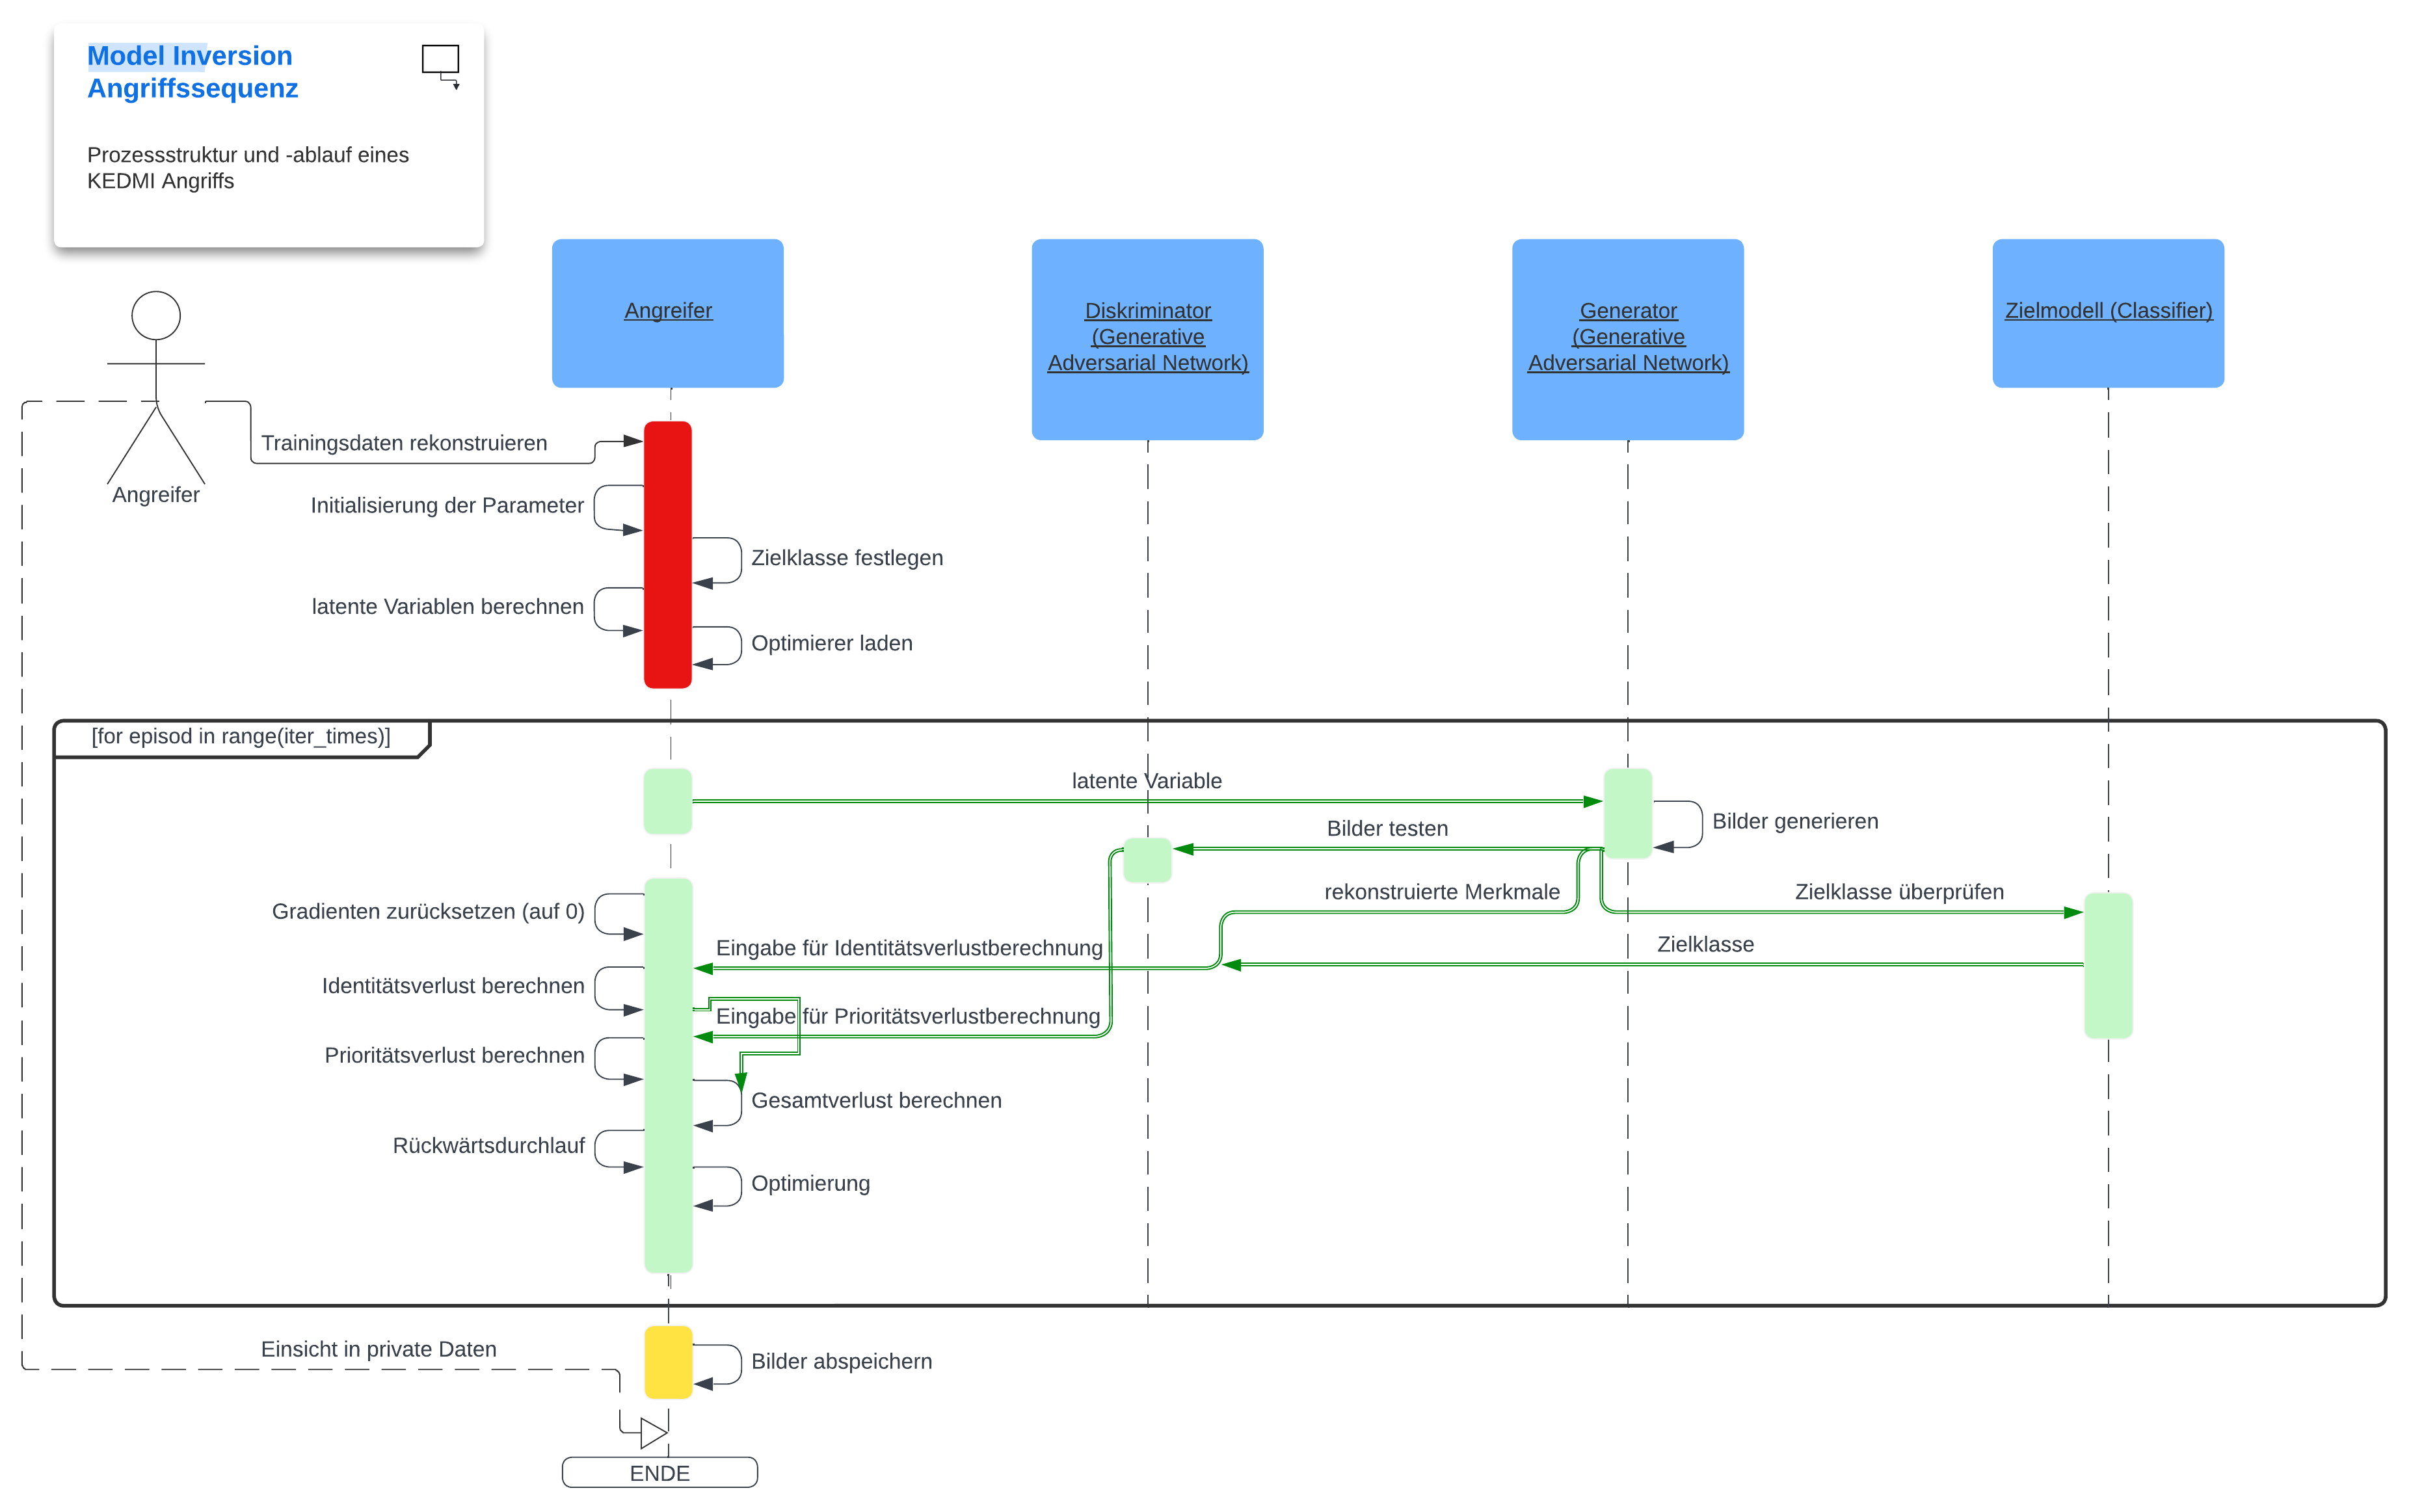
\includegraphics[width=1\linewidth]{Bilder/KEDMI_PROCESS.png}
	\caption{Prozessvisualisierung des KEDMI-Angriffs}
	\label{img:kedmi_process}
\end{figure}

Um diesen Angriff erfolgreich durchzuführen ist es erforderlich nicht nur Zugriff auf das Zielmodell, sondern auch auf einen Generator und seinen zugehörigen Diskriminator zu haben, die für die Generierung und Validierung von Bildern verwendet werden. Der Ablauf des Angriffs, wie in Abbildung \ref{img:kedmi_process} dargestellt, beginnt mit der Initialisierung verschiedener Parameter im Angriffsskript. Zusätzlich muss explizit angegeben werden, welche Klasse rekonstruiert werden soll.

Die resultierenden latenten Variablen spielen im Verlauf des Angriffs eine entscheidende Rolle bei der Rekonstruktion der gewünschten Klassen. Um diese Variablen während des Angriffs präzise anzupassen kommt ein Optimierer zum Einsatz, der die Vektoren in den gewünschten latenten Raum zu optimieren versucht. In der anschließenden Angriffsschleife wird iterativ jeweils ein Bild auf Grundlage der angepassten latenten Variablen erzeugt, das anschließend vom Diskriminator als gefälscht oder real klassifiziert wird. Parallel dazu wird die Zielklasse durch die Eingabe des generierten Bildes in das Zielmodell überprüft.

Anhand dieser ermittelten Variablen werden verschiedene Verluste berechnet, die für die Optimierung des Angriffs verwendet werden. Die Rückwärtsdurchläufe, wie üblicherweise in herkömmlichen Trainingsprozessen verwendet, werden gefolgt von einer Optimierung basierend auf den berechneten Verlusten durchgeführt. Dieser Prozess wiederholt sich über eine vordefinierte Anzahl von Iterationen, wobei in jedem Schritt eine bestimmte Anzahl von Rekonstruktionsbildern erzeugt wird. Diese generierten Bilder werden gespeichert und ermöglichen es dem Angreifer, die Leistung des Angriffs über die Angriffszeit hinweg zu analysieren, indem die Qualität und Genauigkeit der Rückgewinnungen betrachtet werden. Zudem ermöglicht der fortlaufende Analyseprozess dem Angreifer Einsichten in die Wirksamkeit des Angriffs zu erlangen.

Des Weiteren wurde eine Modellinversionsmethode angewandt (\glqq RBMI\grqq{}), die auf dem Prinzip des bestärkenden Lernens durchgeführt wird. Die Implementierungen basieren auf bereits vorhandenene Code-Strukturen des zugrundeliegenden Papers (\cite{han_reinforcement_2023}). Bei dieser Methode werden Konfidenzwerte oder -vektoren der generierten Bilder verwendet, um einem  auf dem \glqq Soft-Actor-Critic-Algorithmus\grqq{} basierenden Agenten Belohnungen zuzuführen. Detailliertere Informationen über diesen lassen sich aus dem entsprechenden Paper entnehmen (\cite{haarnoja_soft_2019}). Der Agent nutzt diese Belohnungen, um private Daten zu rekonstruieren, die während des Trainingsprozesses des Modells verwendet wurden. Aufgrund der begrenzten Zugriffsmöglichkeiten auf das Modell, bei dem der Zugriff auf die Konfidenzwertausgabe des Modells eingeschränkt ist, handelt es sich hierbei um einen sogenannten BlackBox-Angriff.
Der Ansatz des bestärkenden Lernens beinhaltet die Verwendung von Konfidenzwerten, die die Zuversicht oder Sicherheit des Modells in Bezug auf die generierten Daten repräsentieren. Diese Konfidenzwerte dienen als Belohnungen für den Agenten, der daraufhin die Aufgabe hat, die privaten Daten so zu rekonstruieren, dass die Belohnungen maximiert werden.

\begin{figure}
	\centering
	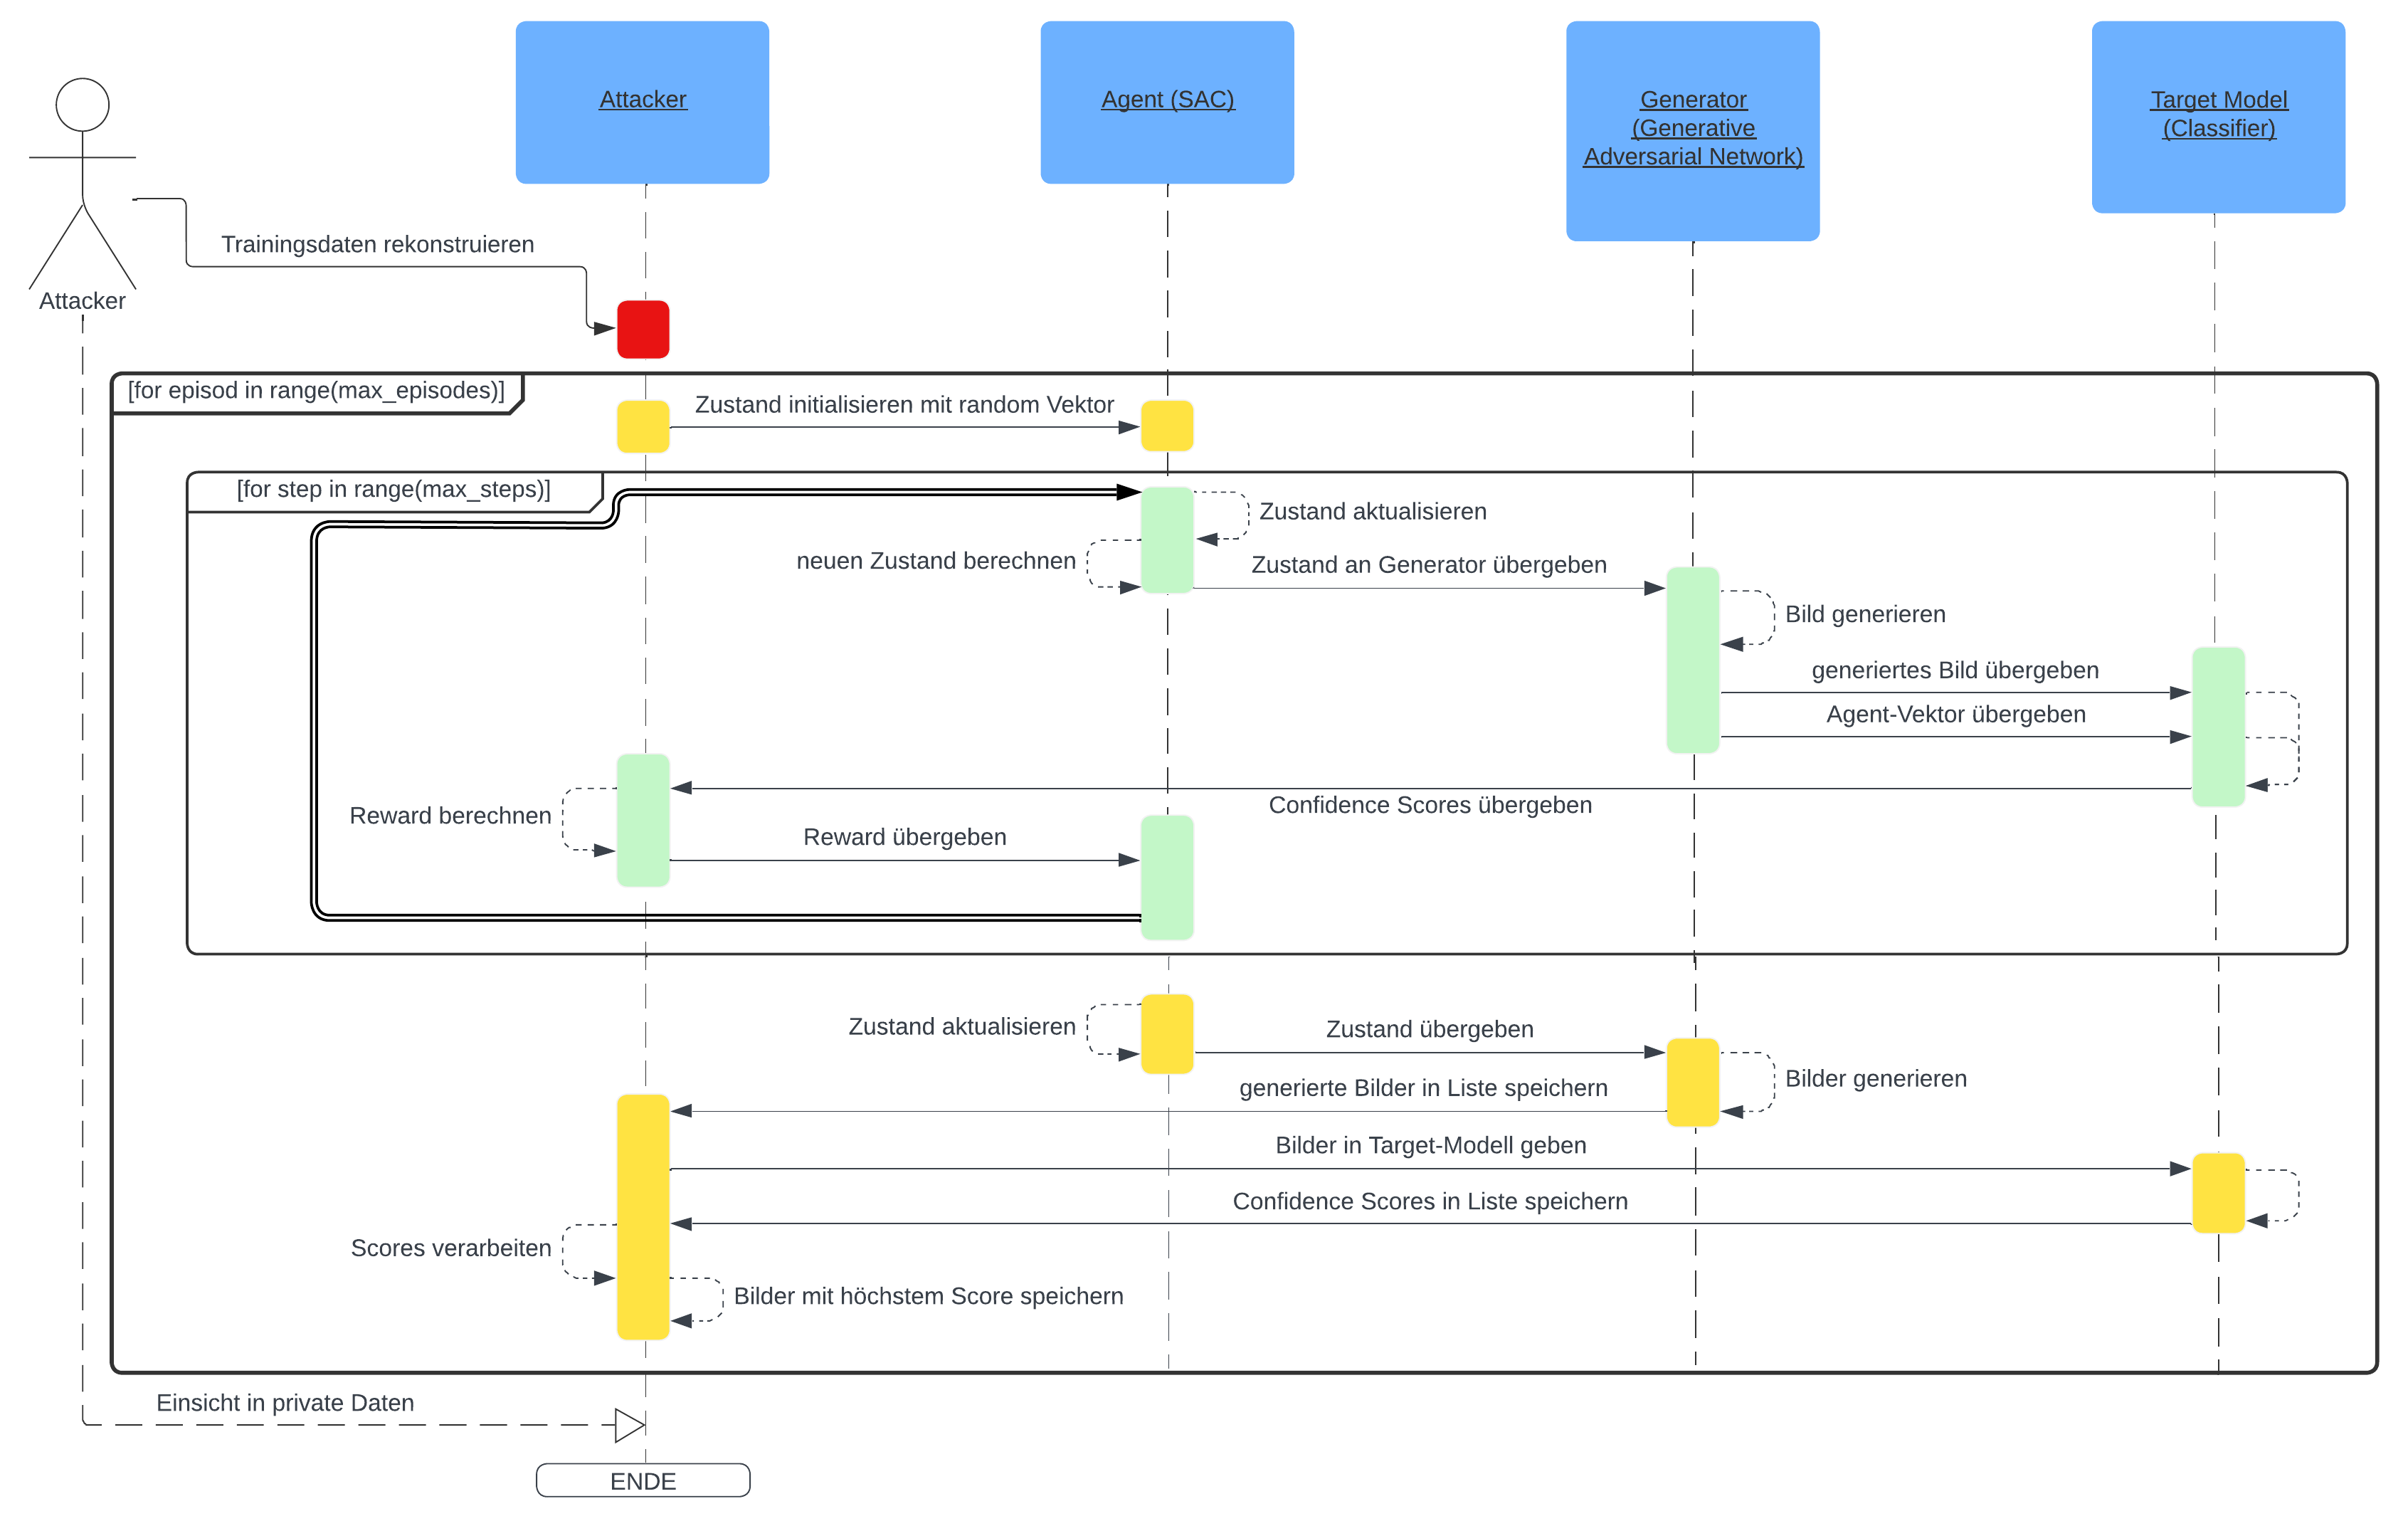
\includegraphics[width=\linewidth]{Bilder/RBMI_PROCESS.png}
	\caption{Prozessvisualisierung des RBMI-Angriffs}
	\label{img:rbmi_process}
\end{figure}

Gemäß der Abbildung \ref{img:rbmi_process} erfordert die Durchführung dieser Attacke neben dem eigentlichen Angriffsskript (dargestellt als Angreifer) Zugriff auf einen Agenten, einen Generator um Bilder der gewünschten Form zu erzeugen, sowie auf ein Zielmodell, das zur Vorhersage eines bestimmten Inputs $I$ verwendet wird. Das Skript des Angreifers ist verantwortlich für die korrekte Ausführung und Verarbeitung verschiedener Werte und Generierungen, um das bestärkende Lernen effektiv zu koordinieren. Der Angriff erfolgt mithilfe mehrerer Schleifen, deren Dauer zu Beginn spezifiziert wird und einen direkten Einfluss auf die Leistung hat.

Mit der Initialisierung des Angriffs wird der Zustand des Agenten mit einem zufälligen Vektor festgelegt, der im Laufe der Ausführungsdauer immer weiter dem zu generierenden Originalbild ähnelt. Um das bestärkende Lernverfahren effektiver durchzuführen, folgt eine Schleife, die über eine vordefinierte Anzahl von Durchgängen läuft. Durch Zustandsaktualisierungen, die auf Belohnungen basieren, wird versucht, dem Originalbild näher zu kommen. Dabei erzeugt der Generator ein bestimmtes Bild auf Basis des aktualisierten Agentenzustands, und der Confidence-Score wird über das Zielmodell berechnet. Ein bestimmter Reward (Belohnung) wird aus diesem Score berechnet, was die nächste Aktualisierung des Agentenzustands beeinflusst und eine Korrektur \glqq in die richtige Richtung\grqq{} veranlasst.

Nach Abschluss der inneren Schleife, die die Zustände dem latenten Vektorraum der Zielklasse anzugleichen versucht, wird der Zustand erneut mit dem bereits beschriebenen Verfahren aktualisiert und das Ergebnis anschließend gespeichert. Auf diese Weise erhält man nach jeder Iteration eine aktualisierte, gespeicherte Momentaufnahme des Angriffsfortschritts sowie der Angriffsqualität. Die Zustandsaktualisierungen basieren immer auf bereits aktualisierte Zustände der vorherigen Iteration.

Nach Abschluss der Ausführung lässt sich das \glqq zurückgenerierte\grqq{} Bild im Verzeichnis der Angriffsergebnisse einsehen.

Dieser Ansatz stellt eine besondere Herausforderung dar, da der Angreifer aufgrund der begrenzten Kenntnis über die internen Strukturen und Parameter des Modells alternative Methoden finden muss, um an sensible Informationen zu gelangen. In diesem Szenario wird bestärkendes Lernen als Mechanismus genutzt, um den Agenten dazu zu bringen, die unsichtbaren Merkmale der generierten Daten zu erlernen und somit private Informationen zu rekonstruieren.
\subsection{Verteidigungsmaßnahmen}
%Differential Privacy
Um den experimentellen Rahmen abzurunden, werden in diesem Abschnitt die implementierten Verteidigungsmaßnahmen präsentiert. Dies beinhaltet Schutzmechanismen, die darauf abzielen, Modelle gegen Angriffe zu stärken und ihre Robustheit zu verbessern. Die Wirksamkeit dieser Verteidigungsstrategien wird kritisch betrachtet und diskutiert.

Für dieses Vorhaben wurde die Methode der differentiellen Privatsphäre, wie in Abschnitt \ref{diff_privacy} beschrieben, eingebunden. Diese Methode zielt darauf ab, Überanpassung (Overfitting) durch das Einbringen von Rauschen in die Trainingsdaten zu verhindern und die erfolgreiche Durchführung von Inferenzangriffen zu erschweren. Die Integration erfolgt mittels des sogenannten Opacus-Frameworks (\cite{noauthor_opacus_nodate}), welches die direkte Implementierung von Trainingsroutinen auf Basis von mit PyTorch erstellten Modellen ermöglicht.

\begin{figure}
	\centering
	\hspace{-1.5cm}
	\includegraphics[width=0.9\linewidth]{Bilder/dpsgd.png}
	\caption{Trainingsprozess eines mit differentieller Privatsphäre durchgeführten Trainings}
	\label{img:dpsgd}
\end{figure}

Im Abbildung \ref{img:dpsgd} wird eine oberflächliche Visualisierung der Trainingsroutine eines neuronalen Netzwerks gezeigt, das auf Basis differentieller Privatsphäre trainiert wird. Dabei wird hervorgehoben, dass sich der Trainingsprozess von dem des \glqq normalen\grqq{} Trainings in verschiedenen Abschnitten durch spezifische Erweiterungen unterscheidet. Diese zusätzlichen Werte repräsentieren allesamt einen besonderen Mehrwert in den zusätzlichen Phasen des DP-SGD-Algorithmus (\cite[3]{abadi_deep_2016}).

Der \textit{Ablauf} des Algorithmus beginnt mit der Initialisierung verschiedener Parameter, die die Rahmenbedingungen des Trainings festlegen. Dazu zählen neben Hyperparametern, wie der Lernrate $\eta_t$, dem Sensitivitätswert $S$, der Gruppierungs- und Rauschgröße ($L$ und $\sigma$), der Gradientenobergrenze $C$ auch die Verlustfunktion 
\begin{equation}
	\mathcal{L}(\theta) = \frac{1}{N} \sum_{i=1} \mathcal{L}(\theta,x_i)
\end{equation}
sowie die Menge der Trainingsdaten $X$ bestehend aus Datenpunkten \{$x_1, x_2, \dots x_n$\}. Auf Basis dieser Werte folgt anschließend eine Schleife über eine bestimmte Epochenanzahl, die auch durch den Trainierenden festgelegt werden muss. In dieser Schleife führt man eine weitere aus, die zufällig über jeden Datenpunkt $x$ iteriert, um auf Basis des Werts verschiedene Operationen auszuführen. Zuerst wird der Gradient auf Basis der angegebenen Verlustfunktion und den aktuellen Modellparametern berechnet: 
\begin{equation}
	g_t(x_i) \leftarrow \nabla_{\theta_t} L(\theta_t, x_i)
\end{equation}
Durch die Berechnung eines Gradienten für jeden einzelnen Datenpunkt kann das Modell auf die spezifischen Eigenschaften angepasst und eine bessere Modellleistung herbeigeführt werden. Im folgenden Schritt wird auf Basis der übergebenen Gradientenobergrenze $C$ der zuvor erechnete Wert angepasst. Das sogenannte \glqq Gradienten-Clipping\grqq{} beschränkt den Datenpunkt der einzelnen Gradienten auf eine bestimmte Größe $C$: 
\begin{equation} 
	g_t(x_i) \leftarrow \frac{g_t(x_i)}{\max \left(1, \frac{\|g_t(x_i)\|_2}{C}\right)}
\end{equation}
Dadurch wird das Problem der explodierenden Gradienten (eng.: Gradient Explosion), das die Leistung und Qualität des Trainings stark beeinflusst, verhindert. Wenn der Wert von $g_t(x_i)$ den Wert $C$ übersteigt, wird dieser durch den Faktor der genannten Formel dividiert. Ein weiterer Vorteil ist dabei die Beschränkung der Sensitivität bezüglich einzelner Datenpunkte, die durch die Oberschwelle $C$ gesteuert werden kann. Je höher diese, desto größer ist das Rauschen, das in folgenden Schritten hinzugefügt werden muss, um den Schutz der Privatsphäre gewährleisten zu können.
Nachdem die Gradienten an das vorgegebene Intervall angepasst wurden, erfolgt die Zugabe von Rauschen zu den Datenpunkten auf Grundlage folgender Formel:
\begin{equation}
	\tilde{g}_t \leftarrow \frac{1}{L} \left( \sum_i \bar{g}_t(x_i) + N(0, \sigma^2C^2I) \right)
\end{equation}
Dabei wird jedem Datenpunkt für den bereits \glqq geclippten\grqq{} Gradienten ein Rauschterm hinzugefügt. Dieser wird durch die Normalverteilung mit Mittelwert 0 und einer Kovarianzmatrix $\Sigma = \sigma^2C^2I $ berechnet. $\sigma$ steht hierbei für die Standardabweichung des Rauschens und $C$ für die Obergrenze des Clippings. Durch das Hinzufügen des Rauschens versucht man die Sensitivität der einzelnen Datenpunkte zu verschleiern und den verstärkten Einfluss bestimmter Parameter auf die Aktualisierung der Modellparameter zu verhindern. Dies hat den Schutz der Privatsphäre zur Folge.

Nach Abschluss sämtlicher Berechnungen für eine festgelegte Anzahl von Datenpunkten, welche durch die Gruppierungsgröße $L$ definiert ist, werden diese zu einem sogenannten Mini-Batch zusammengeführt. Auf Grundlage dieses Mini-Batches erfolgt dann eine Aktualisierung der Modellparameter.

Die Anwendung dieses beschriebenen Prozesses dient dem Schutz der Privatsphäre der während des Trainings verwendeten Datenpunkte. Das wird durch die Vermeidung eines zu großen Einflusses spezifischer Datenpunkte während der Aktualisierung der Modellparameter erreicht.

Die detaillierte Darstellung dieser Elemente bildet das Fundament für die nachfolgenden Experimente und ermöglicht es, die Ergebnisse in einem klaren Kontext zu interpretieren. Die sorgfältige Auswahl und Konfiguration der Experimentierumgebung ist entscheidend für die Zuverlässigkeit und Aussagekraft der gesamten Forschungsarbeit.